% Figure from MATH 591 notes, section 37. Compile with the notes preamble.
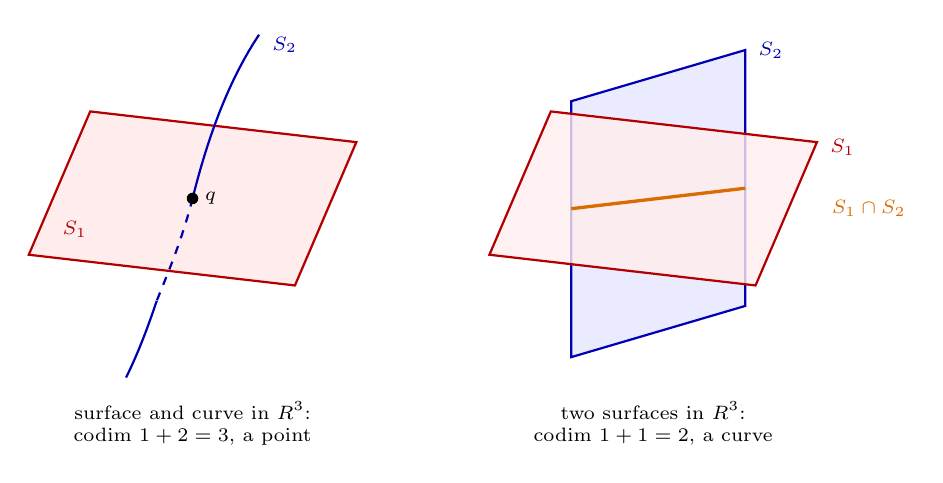
\begin{tikzpicture}[scale=1.3]
\fill[red!7] (0,0.3) -- (2.6,0.0) -- (3.2,1.4) -- (0.6,1.7) -- cycle;
\draw[red!70!black, thick] (0,0.3) -- (2.6,0.0) -- (3.2,1.4) -- (0.6,1.7) -- cycle;
\node[red!70!black, font=\scriptsize] at (0.45,0.55) {$S_1$};
\draw[blue!70!black, thick, dashed] (1.6,0.85) .. controls (1.5,0.45) and (1.35,0.1) .. (1.25,-0.15);
\draw[blue!70!black, thick] (1.25,-0.15) .. controls (1.15,-0.45) and (1.05,-0.7) .. (0.95,-0.9);
\draw[blue!70!black, thick] (1.6,0.85) .. controls (1.75,1.45) and (1.95,2.0) .. (2.25,2.45);
\node[blue!70!black, font=\scriptsize] at (2.5,2.35) {$S_2$};
\fill (1.6,0.85) circle (1.6pt) node[right, font=\scriptsize, xshift=1pt] {$q$};
\node[font=\scriptsize, align=center] at (1.6,-1.35) {surface and curve in $\mathbb{R}^3$:\\ codim $1 + 2 = 3$, a point};
\fill[blue!8] (5.3,-0.7) -- (7.0,-0.2) -- (7.0,2.3) -- (5.3,1.8) -- cycle;
\draw[blue!70!black, thick] (5.3,-0.7) -- (7.0,-0.2) -- (7.0,2.3) -- (5.3,1.8) -- cycle;
\fill[red!7, opacity=0.8] (4.5,0.3) -- (7.1,0.0) -- (7.7,1.4) -- (5.1,1.7) -- cycle;
\draw[red!70!black, thick] (4.5,0.3) -- (7.1,0.0) -- (7.7,1.4) -- (5.1,1.7) -- cycle;
\draw[orange!85!black, very thick] (5.3,0.75) -- (7.0,0.95);
\node[red!70!black, font=\scriptsize] at (7.95,1.35) {$S_1$};
\node[blue!70!black, font=\scriptsize] at (7.25,2.3) {$S_2$};
\node[orange!85!black, font=\scriptsize, anchor=west] at (7.75,0.75) {$S_1 \cap S_2$};
\node[font=\scriptsize, align=center] at (6.1,-1.35) {two surfaces in $\mathbb{R}^3$:\\ codim $1 + 1 = 2$, a curve};
\end{tikzpicture}
